\documentclass{article}

\usepackage{lmodern}
\usepackage[T1]{fontenc}
\usepackage[spanish,activeacute]{babel}
\usepackage{mathtools}
\usepackage{amsmath}
\usepackage{graphicx}
\usepackage[a5paper,margin=1in,top=15mm,bottom=15mm,landscape]{geometry} 
\usepackage{whilecode2}


\graphicspath{ {./imagenes/} }
\title{\textbf{Pr\'actica 3}}
\author{\\Diego Jes\'us Romero Luque}
\date{\today}

\begin{document}
\maketitle
\pagebreak

\begin{enumerate}
  \item Define the TM solution of exercise 3.4 of the problem list and test its correct behaviour.\\
      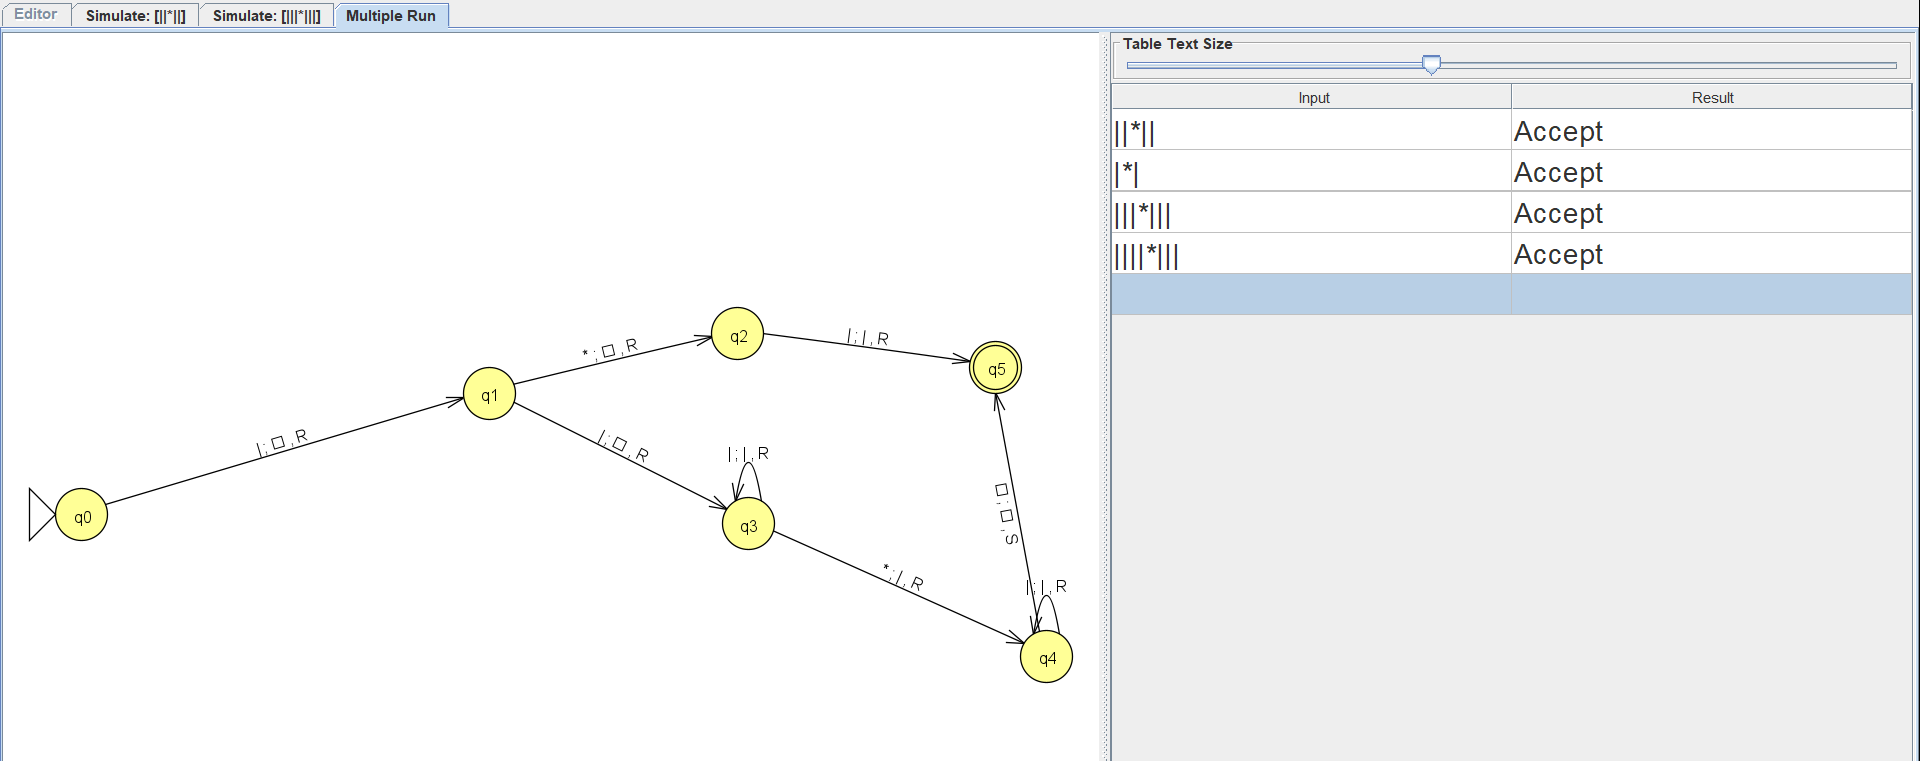
\includegraphics[scale=0.35]{TM.png}
  \pagebreak
  \item Define a recursive function for the sum of three values.
    \begin{center}
      $<$$<\pi^1_1|\sigma(\pi^3_3)>|\sigma(\pi^4_4)>$
    \end{center}
    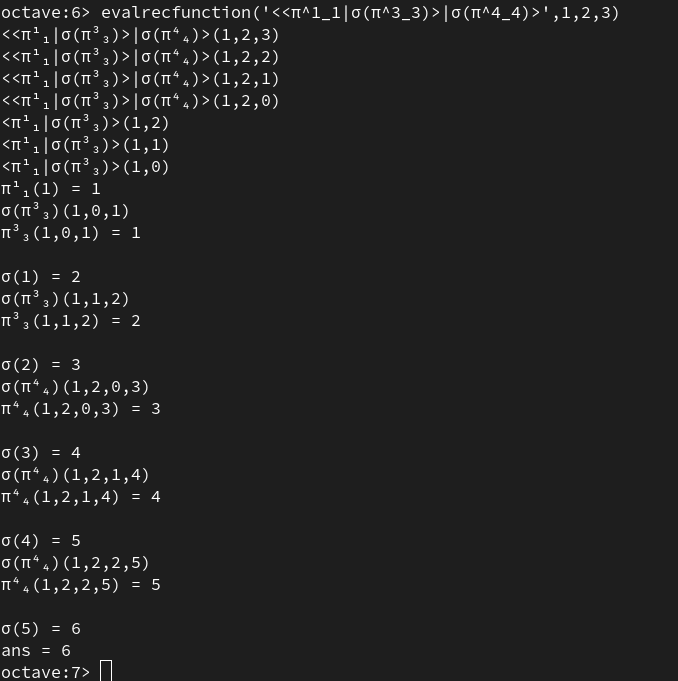
\includegraphics[scale=0.35]{SumaRec.png}
    \pagebreak
  \item Implement a WHILE program that computes the sum of three values. You
   must use an auxiliary variable that accumulates the result of the sum.\\
   \whileprogram{Q}{3}{
    \DefaultVar{4}\Assig\DefaultVar{1}\;
    \While{$X_2 \not = 0$}{
     $X_4 \Assig X_4 + 1$\;
     $X_2 \Assig X_2 - 1$\;
    }
    \While{$X_3 \not = 0$}{
      $X_4 \Assig X_4 + 1$\;
      $X_3 \Assig X_3 - 1$\;
    }
    \DefaultVar{1}\Assig\DefaultVar{4}\;
  }{s}
\end{enumerate}

\end{document}